\id{МРНТИ 65.35.03}

{\bfseries ОПТИМИЗАЦИЯ РЕЦЕПТУРНОГО СОСТАВА БЕЗГЛЮТЕНОВОГО ЗАВАРНОГО
ПОЛУФАБРИКАТА}

{\bfseries \textsuperscript{1}М.Б. Абилова\textsuperscript{\envelope },
\textsuperscript{2}А.М. Омаралиева, \textsuperscript{3}Л.А. Козубаева,
\textsuperscript{1}Ш.К. Байшугулова}

\textsuperscript{1}НАО Казахский агротехнический исследовательский
университет им. С. Сейфуллина, Астана,
Казахстан,\href{https://bankchart.kz/spravochniki/pochtovyye_indeksy/id/116470}{}

\href{https://bankchart.kz/spravochniki/pochtovyye_indeksy/id/116470}{\textsuperscript{2}АО
Казахский университет технологии и бизнеса им. К.Кулажанова, Астана,
Казахстан,}

\href{https://bankchart.kz/spravochniki/pochtovyye_indeksy/id/116470}{\textsuperscript{3}Алтайский
государственный технический университет им. И.И. Позунова, Барнаул,
Россия}

\textsuperscript{\envelope }Корреспондент-автор:
\href{mailto:0909_dm@mail.ru}{\nolinkurl{0909\_dm@mail.ru}}

В кондитерской промышленности сохраняется тенденция роста объемов
производства. В наибольшей степени прирост обеспечивается за счет мучных
кондитерских изделий, удельный вес которых в общем объеме составляет
53,1\%. Создание безглютеновых продуктов является востребованной
областью в пищевой технологии, что обусловлено ростом числа людей,
страдающих от целиакии или непереносимости глютена. Одним из популярных
вариантов безглютеновых кондитерских изделий являются заварные
полуфабрикаты. В статье рассмотрена оптимизация рецептурного состава
заварного полуфабриката с использованием нутовой, кукурузной муки и
меланжа. Проанализирована массовая доля компонентов и их влияние на
удельный объем готового продукта, используя план Шеффе третьего порядка.

Полученные результаты позволили подобрать рецептуру заварного
полуфабриката путем применения разработанной математической модели.

При математическом моделировании показано правильное сочетание нутовой,
кукурузной муки в комбинации с меланжем, которое существенно изменила
свойства заварного полуфабриката.

{\bfseries Ключевые слова:} нутовая мука, кукурузная мука, меланж, план
Шеффе, удельный вес, глютен, заварной полуфабрикат, рецептура.

{\bfseries ГЛЮТЕНСІЗ ҚАЙНАТПАЛЫ ЖАРТЫЛАЙ ФАБРИКАТТЫҢ РЕЦЕПТ ҚҰРАМЫН
ОҢТАЙЛАНДЫРУ}

{\bfseries \textsuperscript{1}М.Б. Абилова\textsuperscript{\envelope },
\textsuperscript{2}А.М. Омаралиева, \textsuperscript{3}Л.А. Козубаева,
\textsuperscript{1}Ш.К. Байшугулова}

\textsuperscript{1}С. Сейфуллин атындағы Қазақ агротехникалық
университеті КеАҚ, Астана, Қазақстан,

\href{https://bankchart.kz/spravochniki/pochtovyye_indeksy/id/116470}{\textsuperscript{2}Қ.
Құлажанов атындағы Қазақ технология және бизнес университеті, Астана,
Қазақстан,}

\href{https://bankchart.kz/spravochniki/pochtovyye_indeksy/id/116470}{\textsuperscript{3}
И. И. Ползунов атындағы Алтай мемлекеттік техникалық университеті},
Барнаул, Ресей,

e-mail: 0909\_dm@mail.ru

Кондитерлік өнеркәсіпте өндіріс көлемінің өсу үрдісі сақталуда. Өсім ең
көп дәрежеде ұн кондитерлік өнімдерінің есебінен қамтамасыз етіледі,
олардың үлес салмағы жалпы көлемде 53,1\% құрайды. Глютенсіз өнімдерді
жасау целиакия ауруы немесе глютенге төзбеушіліктен зардап шегетін
адамдар санының өсуіне байланысты тамақ технологиясында сұранысқа ие
сала болып табылады. Глютенсіз кондитерлік өнімдердің танымал
нұсқаларының бірі-пісірілген жартылай фабрикаттар. Мақалада ноқат,
жүгері ұны мен меланжды қолдана отырып, қайнатылған жартылай фабрикаттың
рецептуралық құрамын оңтайландыру қарастырылады. Үшінші ретті шеффе
жоспарын қолдана отырып, компоненттердің массалық үлесі және олардың
дайын өнімнің меншікті көлеміне әсері талданады.

Алынған нәтижелер әзірленген математикалық модельді қолдану арқылы
қайнатылған жартылай фабрикаттың рецептурасын таңдауға мүмкіндік берді.

Математикалық модельдеу кезінде ноқат, жүгері ұнының меланжмен
үйлесімінде дұрыс үйлесімі көрсетілген, ол қайнатылған жартылай
фабрикаттың қасиеттерін айтарлықтай өзгертті.

{\bfseries Түйін сөздер:} ноқат ұны, жүгері ұны, меланж, шеффе жоспары,
үлес салмағы, глютен, пісірілген жартылай фабрикат, рецепт.

{\bfseries OPTIMIZATION OF THE FORMULATION OF GLUTEN-FREE SEMI-FINISHED
CUSTARD}

{\bfseries \textsuperscript{1}M.B.Abilova\textsuperscript{\envelope },
\textsuperscript{2}A.M. Omaralieva, \textsuperscript{3}L.A. Kozubaeva,
\textsuperscript{1}Sh.K. Baishugulova}

\textsuperscript{1} NJSC «S.Seifullin Kazakh agrotechnical research
University», Astana, Kazakhstan,

\href{https://bankchart.kz/spravochniki/pochtovyye_indeksy/id/116470}{\textsuperscript{2}
K. Kulazhanov Kazakh University of Technology and Business, Astana,
Kazakhstan,}

\href{https://bankchart.kz/spravochniki/pochtovyye_indeksy/id/116470}{\textsuperscript{3}
Altai State Technical University named after I.I. Polzunov, Barnaul,
Russia},

e-mail: \href{mailto:0909_dm@mail.ru}{\nolinkurl{0909\_dm@mail.ru}}

The confectionery industry continues to see an upward trend in
production volumes. To the greatest extent, the increase is provided by
flour confectionery products, the share of which in the total volume is
53.1\%. The creation of gluten-free products is a sought-after area in
food technology, due to the growing number of people suffering from
celiac disease or gluten intolerance. One of the popular options for
gluten-free confectionery products are semi-finished custard products.
The article considers the optimization of the formulation of a
semi-finished custard using chickpea, corn flour and melange. The mass
fraction of the components and their effect on the specific volume of
the finished product are analyzed using the third-order Scheffe plan.

The results obtained made it possible to select the recipe of the
semi-finished custard by applying the developed mathematical model.

Mathematical modeling shows the correct combination of chickpea and corn
flour in combination with melange, which significantly changed the
properties of the semi-finished custard.

{\bfseries Keywords:} chickpea flour, corn flour, melange, Scheffe plan,
specific gravity, gluten, semi-finished custard, recipe.

Введение. Производство специализированных продуктов развивается
стремительными темпами, в частности продуктов питания, которые
освобождены от определенных ингредиентов, не рекомендованных по
медицинским показаниям некоторым группам населения. Это могут быть
аллергены, олигосахариды и некоторые типы белков.

В настоящее время сегмент рынка специализированных пищевых продуктов
питания расширяется. У людей, которым жизненно необходимы такие продукты
питания, появляется возможность употребления пищи без ущемления своих
вкусовых пристрастий и потребностей, а также возможность разнообразить
свой дневной рацион за счет основных и дополнительных блюд. Большую
часть рынка продуктов специализированного назначения занимают продукты
импортного производства. К специализированным продуктам питания относят
продукты, не содержащие глютен и рекомендованные людям, страдающим
целиакией (непереносимостью глютена) {[}1{]}.

Безглютеновая продукция должна соответствовать строгим стандартам, чтобы
обеспечить потребителю не только безопасность, но и вкусовые качества.
Разработка таких изделий требует внимания к выбору компонентов, их
взаимодействию и технологии обработки.

Одним из ключевых факторов, влияющих на качество безглютенового
заварного полуфабриката, является структура его матрицы. Комплексные
взаимодействия между различными видами муки и другими ингредиентами
определяют не только текстуру, но и прочность, пористость и вкус
готового изделия.

Оптимизация рецептуры безглютенового заварного полуфабриката позволяет
не только улучшить его органолептические и текстурные свойства, но и
создать продукт с высокой питательной ценностью. Важно учитывать не
только количественные аспекты, но и качество исходных материалов.

Нутовая мука, получаемая из свежего или сухого нута, является богатым
источником белка и клетчатки. Ее использование в безглютеновых рецептах
способствует не только улучшению пищевой ценности, но и обогащению
продукта витаминными и минеральными компонентами.

Как показывает практика, нутовая мука обладает способности к образованию
жидкостной матрицы, что позитивно сказывается на удержании влаги и
формировании структуры теста. В семенах нута содержание жира достигает
8\% и характерезируется наличием в нем жирных кислот. Наиболее важные из
них -- линолевая и олеиновая кислота, которые необходимы для человеку
для осуществления ростовых процессов и различных физиологических
функций. Они не синтезируется в организме человека, поэтому поддержание
уровня этих кислот зависит только от поступления их с пищей {[}2{]}.

Однако важно отметить, что она имеет специфический вкус, который может
влиять на конечный продукт. Оптимальные массовые доли нутовой муки в
рецептуре определяются через экспериментальные исследования. Кукурузная
мука является еще одним популярным компонентом в безглютеновом
производстве. Она отличается легкостью и нейтральным вкусом, что делает
ее идеальным дополнением к другим видам муки. Кукурузная мука
способствует улучшению структуры теста, а также повышает его
органолептические свойства. Заварной полуфабрикат с заменой пшеничной
муки кукурузной на 50\% характеризуется высокими органолептическими
показателями: он имеет правильную форму с небольшими трещинами на
поверхности, большой объем и внутри образуется большая полость {[}3{]}.

В процессе опытов по оптимизации рецептуры было установлено, что
кукурузная мука взаимодействует с нутовой, создавая определенные
текстурные и вкусовые характеристики. Ключевым моментом является баланс
между этими двумя компонентами.

Высокое содержание кукурузной муки может привести к утрате питательных
свойств, в то время как недостаток может негативно сказаться на
текстуре. Молекулы глютелина кукурузы не способны образовывать
непрерывную структуру в тесте вследствие наличия большого количества
поперечных связей между молекулами белка. Количество глютелиновой
фракции, экстрагируемой 0,2 \%-ным раствором едкого натрия, в
значительной степени зависит от условий предшествующей экстракции:
применение смеси 70 \%-ного раствора этанола с уксуснокислым натрием
понижает выход глютелиновой фракции по сравнению с экстракцией чистым
этанолом. Поэтому в нашей работе кукурузная мука используется для
улучшения качества, а также увеличения пищевой ценности и уменьшения
калорийности мучных кондитерских изделий {[}4{]}.

Меланж, представляющий собой смесь яиц и яичного порошка, в современных
рецептурах используется для улучшения структуры и текстуры. Он не только
увеличивает питательную ценность продукта, но и способствует улучшению
его вкусовых качеств.

В исследуемых рецептурах меланж играет важную роль в формировании
воздушности и легкости полуфабриката. Однако влияние массовой доли
меланжа на удельный объем продукта также требует внимания. Лишнее
количество этого компонента может негативно сказаться на конечном
результате, что подчеркивает важность нахождения оптимальных пропорций
{[}5,6{]}.

Во многих процессах, связанных с пищевыми продуктами, в продуктах
происходят значительные изменения объема и большая деформация. Типичные
примеры: усадка фруктов и овощей во время конвективной сушки и мясных
продуктов во время приготовления, расширение хлеба во время выпекания,
расширение при экструзии. В некоторых случаях эти явления являются
положительными и действительно являются характерной чертой процесса,
например, расширение при выпечке и экструзии. С другой стороны, они
могут представлять собой нежелательные изменения в других ситуациях,
например, чрезмерную усадку во время сушки и приготовления пищи. Однако
в любом случае для широкого круга процессов, условий эксплуатации и
пищевых материалов значительное изменение объема и деформация являются
частью процессов и, таким образом, неизбежны. Следовательно, необходимо
лучше понять фундаментальные механизмы этих явлений в контексте пищевой
инженерии, то есть развивать научные знания и полезные инструменты для
описания и прогнозирования взаимосвязей между условиями обработки и
поведением пищевых материалов {[}7,8{]}.

Математическое моделирование рецептуры при создании нового
безглютенового кондитерского изделия имеет несколько ключевых
преимуществ такие как оптимизация ингредиентов, прогнозирование
результатов, экономия результатов, анализ свойств, индивидуальный
подход.

Использование математического моделирования в разработке безглютеновых
кондитерских изделий делает процесс более научным и систематизированным,
что увеличивает шансы на успех в создании новых и вкусных продуктов
{[}7,8,9{]}.

Из вышеизложенного вытекает необходимость решения задачи применения
математической обработки для создания рецептуры на основе зернобобовых и
злаковых культур.

Материалы и методы. Для оптимизации рецептуры был разработан
экспериментальный план на основе метода Шеффе третьего порядка. Данный
подход позволяет эффективно варьировать массовые доли нутовой муки (х1),
кукурузной муки (х2) и меланжа (х3), сохраняя при этом контроль над
другими параметрами {[}10{]}.

Переменными факторами при составлении рецептуры выступали массовые доли
нутовой муки (\emph{х\textsubscript{1}}), кукурузной муки
(\emph{х\textsubscript{2}}) и меланжа (\emph{х\textsubscript{3}}) в
составе рецептуры. Эти факторы варьировали в соответствии с планом Шеффе
третьего порядка. Другие условия опытов оставались неизменными.
Результаты опытов характеризовали изменение одного из показателей --
удельный объем.

Компоненты заварного полуфабриката, образующие матрицу планирования, и
результаты опытов приведены в таблице 1.

{\bfseries Таблица 1 - План Шеффе и результаты опытов}

% \begin{longtable}[]{@{}
%   >{\raggedright\arraybackslash}p{(\columnwidth - 14\tabcolsep) * \real{0.1243}}
%   >{\raggedright\arraybackslash}p{(\columnwidth - 14\tabcolsep) * \real{0.0906}}
%   >{\raggedright\arraybackslash}p{(\columnwidth - 14\tabcolsep) * \real{0.0850}}
%   >{\raggedright\arraybackslash}p{(\columnwidth - 14\tabcolsep) * \real{0.1112}}
%   >{\raggedright\arraybackslash}p{(\columnwidth - 14\tabcolsep) * \real{0.1060}}
%   >{\raggedright\arraybackslash}p{(\columnwidth - 14\tabcolsep) * \real{0.1060}}
%   >{\raggedright\arraybackslash}p{(\columnwidth - 14\tabcolsep) * \real{0.1060}}
%   >{\raggedright\arraybackslash}p{(\columnwidth - 14\tabcolsep) * \real{0.2710}}@{}}
% \toprule\noalign{}
% \multirow{3}{=}{\begin{minipage}[b]{\linewidth}\raggedright
% Номера опытов
% \end{minipage}} &
% \multicolumn{6}{>{\raggedright\arraybackslash}p{(\columnwidth - 14\tabcolsep) * \real{0.6048} + 10\tabcolsep}}{%
% \begin{minipage}[b]{\linewidth}\raggedright
% Массовая доля компонентов
% \end{minipage}} &
% \multirow{2}{=}{\begin{minipage}[b]{\linewidth}\raggedright
% Удельный объем, см\textsuperscript{3}/мг
% \end{minipage}} \\
% &
% \multicolumn{3}{>{\raggedright\arraybackslash}p{(\columnwidth - 14\tabcolsep) * \real{0.2868} + 4\tabcolsep}}{%
% \begin{minipage}[b]{\linewidth}\raggedright
% Кодированные значения
% \end{minipage}} &
% \multicolumn{3}{>{\raggedright\arraybackslash}p{(\columnwidth - 14\tabcolsep) * \real{0.3180} + 4\tabcolsep}}{%
% \begin{minipage}[b]{\linewidth}\raggedright
% Натуральные значения
% \end{minipage}} \\
% & \begin{minipage}[b]{\linewidth}\raggedright
% \emph{х\textsubscript{1}}
% \end{minipage} & \begin{minipage}[b]{\linewidth}\raggedright
% \emph{х\textsubscript{2}}
% \end{minipage} & \begin{minipage}[b]{\linewidth}\raggedright
% \emph{х\textsubscript{3}}
% \end{minipage} & \begin{minipage}[b]{\linewidth}\raggedright
% НМ, u
% \end{minipage} & \begin{minipage}[b]{\linewidth}\raggedright
% КМ, г
% \end{minipage} & \begin{minipage}[b]{\linewidth}\raggedright
% М, г
% \end{minipage} & \begin{minipage}[b]{\linewidth}\raggedright
% \emph{у}
% \end{minipage} \\
% \midrule\noalign{}
% \endhead
% \bottomrule\noalign{}
% \endlastfoot
% 1 & 1 & 0 & 0 & 54,0 & 0,0 & 0,0 & 9,7 \\
% 2 & 2/3 & 1/3 & 0 & 35,6 & 18,0 & 0,0 & 10,2 \\
% 3 & 2/3 & 0 & 1/3 & 35,6 & 0,0 & 18,0 & 10,2 \\
% 4 & 1/3 & 2/3 & 0 & 18,0 & 35,6 & 0,0 & 10,5 \\
% 5 & 1/3 & 1/3 & 1/3 & 18,0 & 18,0 & 18,0 & 10,8 \\
% 6 & 1/3 & 0 & 2/3 & 18,0 & 0,0 & 35,6 & 10,6 \\
% 7 & 0 & 1 & 0 & 0,0 & 54,0 & 0,0 & 10,4 \\
% 8 & 0 & 2/3 & 1/3 & 0,0 & 35,6 & 18,0 & 10,7 \\
% 9 & 0 & 1/3 & 2/3 & 0,0 & 18,0 & 35,6 & 10,9 \\
% 10 & 0 & 0 & 1 & 0,0 & 0,0 & 54,0 & 10,8 \\
% \end{longtable}

Оценочные эффекты полной модели для удельного объема представлены в
таблице 2

{\bfseries Таблица 2 - Оценочные эффекты полной модели для удельного
объема}

% \begin{longtable}[]{@{}
%   >{\raggedright\arraybackslash}p{(\columnwidth - 10\tabcolsep) * \real{0.1895}}
%   >{\raggedright\arraybackslash}p{(\columnwidth - 10\tabcolsep) * \real{0.2120}}
%   >{\raggedright\arraybackslash}p{(\columnwidth - 10\tabcolsep) * \real{0.1078}}
%   >{\raggedright\arraybackslash}p{(\columnwidth - 10\tabcolsep) * \real{0.1854}}
%   >{\raggedright\arraybackslash}p{(\columnwidth - 10\tabcolsep) * \real{0.1334}}
%   >{\raggedright\arraybackslash}p{(\columnwidth - 10\tabcolsep) * \real{0.1718}}@{}}
% \toprule\noalign{}
% \endhead
% \bottomrule\noalign{}
% \endlastfoot
% Значения & Сумма квадратов & Различие & Средний квадрат & F-отношение &
% Значение Р \\
% Средний & 1098,3 & 1 & 1098,3 & & \\
% Линейный & 0,985334 & 2 & 0,492667 & 14,95 & 0,0030 \\
% Квадратичный & 0,205143 & 3 & 0,0683809 & 10,72 & 0,0221 \\
% Специальный кубический & 0,0209994 & 1 & 0,0209994 & 13,93 & 0,0335 \\
% Кубический & 0,00452394 & 3 & 0,00150798 & & \\
% Ошибка & -1,01163E-13 & 0 & 0 & & \\
% Итого & 1099,52 & 10 & & & \\
% \end{longtable}

В таблице 2 показаны результаты подгонки различных моделей к данным
удельного объема. Средняя модель состоит только из константы. Линейная
модель состоит из членов первого порядка для каждой из компонент.
Квадратичная модель добавляет перекрестные произведения между парами
компонентов. Специальная кубическая модель добавляет термины, включающие
произведения трех компонентов. Кубическая модель добавляет другие члены
третьего порядка. Каждая модель показана с P-значением, которое
проверяет, является ли эта модель статистически значимой по сравнению со
средним квадратом для приведенного ниже термина. Обычно выбирают самую
сложную модель с P-значением менее 0,05, предполагая, что работа
выполняется на уровне достоверности 95,0\%. К сожалению, нет степеней
свободы для ошибки, поэтому статистическую значимость кубической модели
проверить невозможно. Добавление дополнительных запусков в дизайн
облегчит эту проблему. Текущая выбранная модель --- это специальная
кубическая модель, дисперсионный анализ приведенная в таблице 3.

{\bfseries Таблица 3 - Дисперсионный анализ удельного объема заварного
полуфабриката (ANOVA)}

% \begin{longtable}[]{@{}
%   >{\raggedright\arraybackslash}p{(\columnwidth - 10\tabcolsep) * \real{0.1895}}
%   >{\raggedright\arraybackslash}p{(\columnwidth - 10\tabcolsep) * \real{0.2120}}
%   >{\raggedright\arraybackslash}p{(\columnwidth - 10\tabcolsep) * \real{0.1078}}
%   >{\raggedright\arraybackslash}p{(\columnwidth - 10\tabcolsep) * \real{0.1854}}
%   >{\raggedright\arraybackslash}p{(\columnwidth - 10\tabcolsep) * \real{0.1334}}
%   >{\raggedright\arraybackslash}p{(\columnwidth - 10\tabcolsep) * \real{0.1718}}@{}}
% \toprule\noalign{}
% \endhead
% \bottomrule\noalign{}
% \endlastfoot
% Значения & Сумма квадратов & Различие & Средний квадрат & F-отношение &
% Значение Р \\
% Специальная кубическая модель & 1,21148 & 6 & 0,201913 & 133,90 &
% 0,0010 \\
% Total error & 0,00452394 & 3 & 0,00150798 & & \\
% Total (corr.) & 1,216 & 9 & & & \\
% \end{longtable}

В таблице 3 показан дисперсионный анализ для текущей выбранной
специальной кубической модели. Поскольку P-значение для этой модели
меньше 0,05, существует статистически значимая связь между удельным
объемом и компонентами на уровне достоверности 95,0\%.

Тест на несоответствие предназначен для определения того, адекватна ли
выбранная модель для описания наблюдаемых данных или следует
использовать более сложную модель. Тест выполняется путем сравнения
изменчивости невязок текущей модели с изменчивостью между наблюдениями
при повторных настройках компонентов. К сожалению, в этом случае
провести тест невозможно, так как нет повторных наблюдений.

Статистика R-квадрата показывает, что подобранная модель объясняет
99,628\% изменчивости удельного объема в зависимости от компонентов
заварного полуфабриката. Скорректированная статистика R-квадрата,
которая больше подходит для сравнения моделей с разным количеством
независимых переменных, составляет 98,8839\%. Стандартная ошибка оценки
показывает, что стандартное отклонение остатков составляет 0,0388327.
Средняя абсолютная ошибка (MAE) 0,0176194 является средним значением
остатков. Статистика Дарбина-Ватсона (DW) проверяет остатки, чтобы
определить, существует ли какая-либо существенная корреляция на основе
порядка, в котором они встречаются в данных. Поскольку P-значение больше
5,0\%, нет никаких указаний на серийную автокорреляцию в остатках на
уровне значимости 5,0\%. Результаты подбора специальной кубической
модели для удельного объема и коэффициенты регрессии приведены в таблице
4.

{\bfseries Таблица 4 - Результаты подбора специальной кубической модели для
удельного объема}

% \begin{longtable}[]{@{}
%   >{\raggedright\arraybackslash}p{(\columnwidth - 4\tabcolsep) * \real{0.3639}}
%   >{\raggedright\arraybackslash}p{(\columnwidth - 4\tabcolsep) * \real{0.3030}}
%   >{\raggedright\arraybackslash}p{(\columnwidth - 4\tabcolsep) * \real{0.3332}}@{}}
% \toprule\noalign{}
% \endhead
% \bottomrule\noalign{}
% \endlastfoot
% Компоненты & Коэффициенты & Ошибка \\
% A:Нутовая мука & 9,68571 & 0,0369373 \\
% B:Кукурузная мука & 10,4 & 0,0369373 \\
% C:Меланж & 10,8143 & 0,0369373 \\
% \end{longtable}

Таким образом, зависимость удельного объема от компонентов заварного
полуфабриката может быть представлена в виде массовой доли ингредиентов
по отдельности, и уравнение регрессии можно записать в следующем виде:

\emph{y} = 9,68571\emph{х\textsubscript{1 }}+
10,4\emph{х\textsubscript{2}}+ 10,8143\emph{х\textsubscript{3}}+
1,38214\emph{х\textsubscript{1}х\textsubscript{2}}+

0,674999\emph{х\textsubscript{1}х\textsubscript{3}}+
0,867856\emph{х\textsubscript{2}х\textsubscript{3}}+
4,72439\emph{х\textsubscript{1}х\textsubscript{2}х\textsubscript{3}}

{\bfseries Результаты их обсуждения.} На основании полученной уравнения
регрессии построили модель в трехмерном пространстве, представляющую
собой плоскость, которая характеризует зависимость удельного объема
заварного полуфабриката от компонентов. На рисунках 1-4 приведены
графические изображения графиков зависимостей.

\begin{figure}[H]
	\centering
	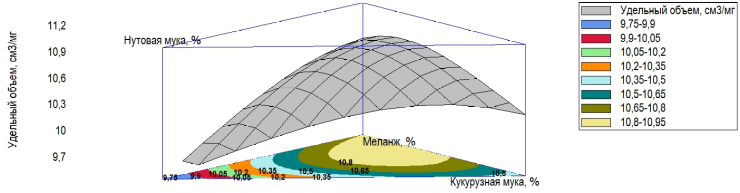
\includegraphics[width=0.8\textwidth]{media/pish/image1}
	\caption*{}
\end{figure}


{\bfseries Рис. 1 - Поверхность отклика выходного параметра -- зависимость
удельного объема от массовой доли компонентов}

\begin{figure}[H]
	\centering
	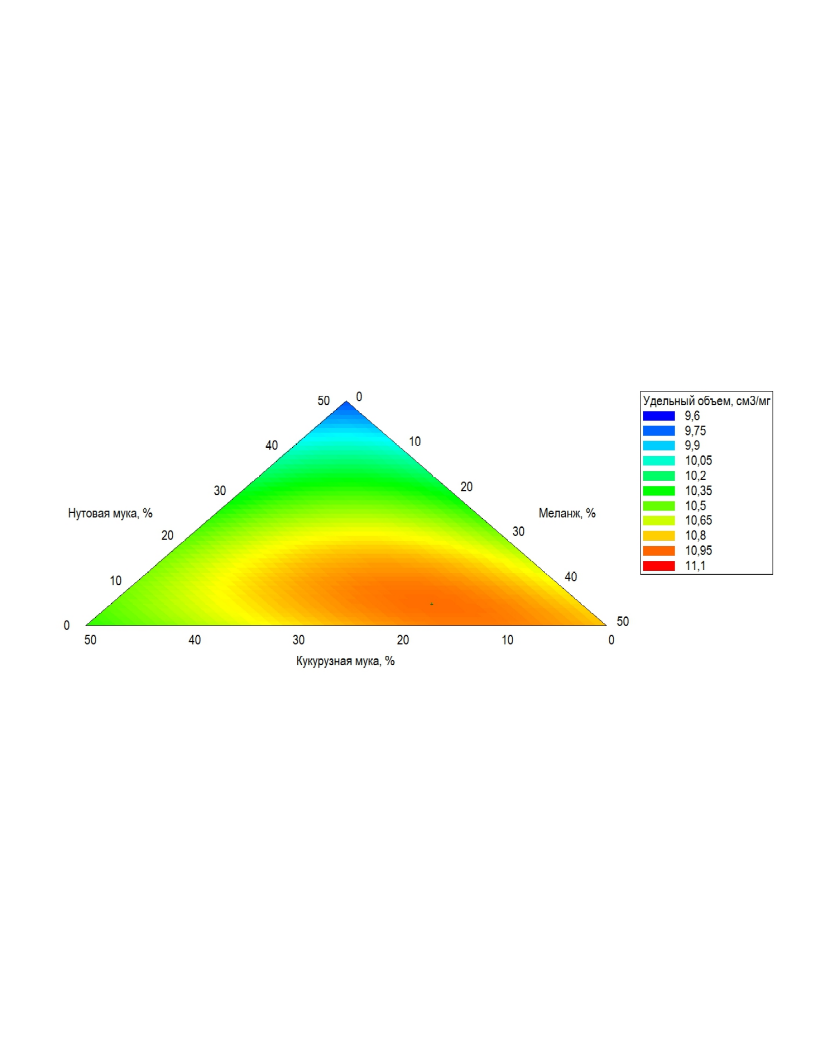
\includegraphics[width=0.8\textwidth]{media/pish/image2}
	\caption*{}
\end{figure}


{\bfseries Рис. 2 - Проекции сечений поверхности отклика, характеризующие
зависимость удельного объема от массовой доли компонентов}

\begin{figure}[H]
	\centering
	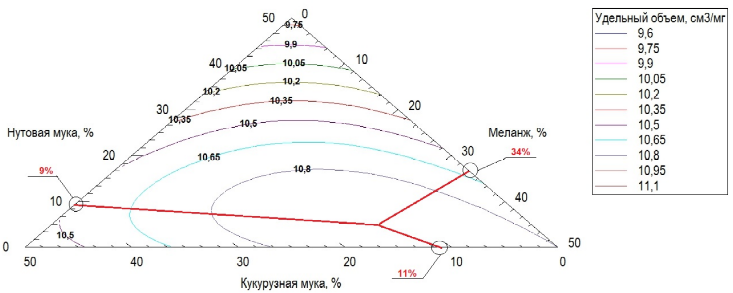
\includegraphics[width=0.8\textwidth]{media/pish/image3}
	\caption*{}
\end{figure}


{\bfseries Рис. 3 - Проекции сечений поверхности отклика, характеризующие
зависимость удельного объема от массовой доли компонентов с оптимальными
точками}

\begin{figure}[H]
	\centering
	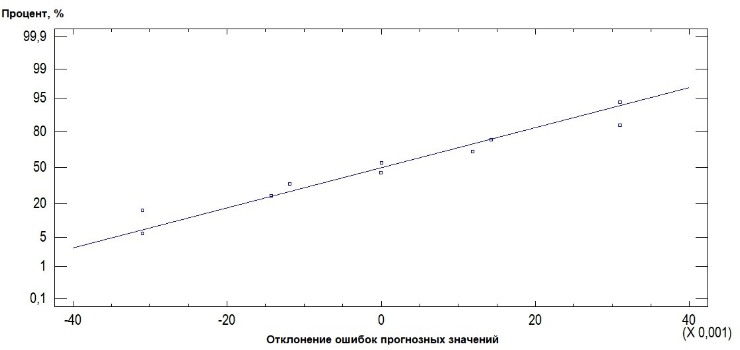
\includegraphics[width=0.8\textwidth]{media/pish/image4}
	\caption*{}
\end{figure}


{\bfseries Рис. 4 - График диагностики отклонения ошибок прогноза значений}

{\bfseries удельного объема от нормального распределения}

Анализ поведения полученной поверхности откликов показал, что
оптимальной зоной удельного объема заварного полуфабриката, достигаются,
когда массовое доля нутовой муки составит 9\%, массовое доля кукурузной
муки 11\% и массовое доля меланжа 34\%. Анализ распределения ошибок
прогноза значений удельного объема дал удовлетворительные результаты:
значительные часть точек заметно не отклонились от прямой, что дает
адекватность полученной модели.

{\bfseries Выводы.} Полученные результаты позволили подобрать рецептуру
заварного полуфабриката путем применения разработанной математической
модели.

При пересчете на 1000 г продукта в натуральном значений рецептура
заварного полуфабриката выглядит таким образом:

- нутовая мука -- 90 г;

- кукурузная мука -- 110 г;

- меланж -- 340 г.

Таким образом, исследования показывают, что правильное сочетание нутовой
и кукурузной муки в комбинации с меланжем может существенно изменить
свойства заварного полуфабриката. Оптимизация рецептуры является
процессом, требующим учета множества факторов, но результаты явно
свидетельствуют о возможности создания качественного безглютенового
продукта, соответствующего современным требованиям рынка.

{\bfseries Литература}

\begin{enumerate}
\def\labelenumi{\arabic{enumi}.}
\item
  Пикулина Н.С., Резниченко И.Ю. Обзор рынка безглютеновых мучных
  кондитерских изделий// Пищевые инновации в биотехнологии // Сборник
  тезисов VI Международной научной конференции студентов, аспирантов и
  молодых ученых. Том 2. Под общей редакцией А.Ю. Просекова. 2018.-
  С.355-356.
\item
  Зернобобовые культуры в структуре функционального питания (фасоль
  зерновая и овощная, горох овощной, нут). -2019. -№. 133. - С. 157-167.
\end{enumerate}

DOI: 10.36305/0513-1634-2019-133-157-167

\begin{enumerate}
\def\labelenumi{\arabic{enumi}.}
\setcounter{enumi}{2}
\item
  Ушакова С.Г., Лунева О.Н. Обоснование использования кукурузной муки в
  технологии заварного полуфабриката //Новые концептуальные подходы к
  решению глобальной проблемы обеспечения продовольственной безопасности
  в современных условиях // сборник научных статей 9-й Международной
  научно-практической конференции. Юго-Западный государственный
  университет. Курск. - 2021. - С. 462 - 464.
\item
  Корячкина, С. Я., Матвеева Т.В. Новые виды мучных и кондитерских
  изделий. Научные основы, технологии, рецептуры. -Орел: Труд, 2006. -С.
  178-179. ISBN: 5-89436-066-8
\item
  Качество и безопасность пищевой продукции по системе ХАССП (Яичный
  меланж). -2021. -№ 9. URL:
  https://cyberleninka.ru/article/n/kachestvo-i-bezopasnost-pischevoy-produktsii-po-sisteme-hassp-yaichnyy-melanzh
\item
  Корроль А.Е., Дроздова Л.И. Меланж как продукт пищевой промышленности
  // Молодежь и наука. -2017. -С. 27. ISSN: 2308-0426
\item
  Ломакина П.А., Фролов Д.И. Обзор современных тенденций в моделировании
  процессов происходящих при обработке пищевых продуктов //
  Инновационная техника и технология. -2023. -Т. 10. -№ 1. -С. 73-80.
\item
  Ахмадиев Ф.Г., Р.М. Гильфанов Математическое моделирование и
  оптимизация «состав свойство» многокомпонентных смесей // Известия
  КГАСУ. -2012. -№ 2(20). -С. 289-297.
\item
  Ho, Q. T., Carmeliet, J., Datta, A. K., Defraeye, T., Delele, M. A.,
  Herremans, E., Opara, L., Ramon, H., Tijskens, E., van der Sman, R. G.
  M., Van Liedekerke, P., Verboven, P., \& Nicolai, B. M. Multiscale
  modeling in food engineering. // Journal of Food Engineering - 2013.
  -114(3), P. 279-291. DOI: 10.1016/j.jfoodeng.2012.08.019
\item
  Протасевич Г.Ф., Мельниченко В.В., Смёткин В.А., Михлюк А.И. Основы
  научных исследовании. Математическое моделирование технологических
  процессов// Учебно-методическое пособие//БНТУ.- Минск, 2009. -Ч.1. -С.
  73-79.
\item
  URL: https://rep.bntu.by/handle/data/5233
\end{enumerate}

{\bfseries References}

1.Pikulina N.S., Reznichenko I.Ju. Obzor rynka bezgljutenovyh muchnyh
konditerskih izdelij// Pishhevye innovacii v biotehnologii // Sbornik
tezisov VI Mezhdunarodnoj nauchnoj konferencii studentov, aspirantov i
molodyh uchenyh. Tom 2. Pod obshhej redakciej A.Ju. Prosekova. 2018. -
S.355- 356. {[}in Russian{]}

2.Zernobobovye kul' tury v strukture
funkcional' nogo pitanija (fasol'{}
zernovaja i ovoshhnaja, goroh ovoshhnoj, nut). -2019. -№. 133. -S.
157-167. DOI: 10.36305/0513-1634-2019-133-157-167 {[}in Russian{]}

3.Ushakova S.G., Luneva O.N. Obosnovanie ispol' zovanija
kukuruznoj muki v tehnologii zavarnogo polufabrikata //Novye
konceptual' nye podhody k resheniju
global' noj problemy obespechenija
prodovol' stvennoj bezopasnosti v sovremennyh uslovijah
// sbornik nauchnyh statej 9-j Mezhdunarodnoj nauchno-prakticheskoj
konferencii. Jugo-Zapadnyj gosudarstvennyj universitet. Kursk. - 2021.-
S. 462- 464. {[}in Russian{]}

4.Korjachkina, S. Ja., Matveeva T.V. Novye vidy muchnyh i konditerskih
izdelij. Nauchnye osnovy, tehnologii, receptury. -Orel: Trud, 2006. -S.
178-179. ISBN: 5-89436-066-8 {[}in Russian{]}

5.Kachestvo i bezopasnost'{} pishhevoj produkcii po
sisteme HASSP (Jaichnyj melanzh). -2021. -№ 9. URL:
https://cyberleninka.ru/article/n/kachestvo-i-bezopasnost-pischevoy-produktsii-po-sisteme-hassp-yaichnyy-melanzh
{[}in Russian{]}

6.Korrol'{} A.E., Drozdova L.I. Melanzh kak produkt
pishhevoj promyshlennosti // Molodezh'{} i nauka. -2017.
-S. 27. ISSN: 2308-0426 {[}in Russian{]}

7.Lomakina P.A., Frolov D.I. Obzor sovremennyh tendencij v modelirovanii
processov proishodjashhih pri obrabotke pishhevyh produktov //
Innovacionnaja tehnika i tehnologija. -2023. -T. 10. -№ 1. -S. 73 - 80.
{[}in Russian{]}

8.Ahmadiev F.G., R.M. Gil' fanov Matematicheskoe
modelirovanie i optimizacija «sostav svojstvo» mnogokomponentnyh smesej
// Izvestija KGASU. -2012. -№ 2(20). -S. 289-297. {[}in Russian{]}

9. Ho, Q. T., Carmeliet, J., Datta, A. K., Defraeye, T., Delele, M. A.,
Herremans, E., Opara, L., Ramon, H., Tijskens, E., van der Sman, R. G.
M., Van Liedekerke, P., Verboven, P., \& Nicolai, B. M. Multiscale
modeling in food engineering. // Journal of Food Engineering --2013.
--114(3), P. 279-291. DOI 10.1016/j.jfoodeng.2012.08.019 {[}in
Russian{]}

10.Protasevich G.F., Mel' nichenko V.V., Smjotkin V.A.,
Mihljuk A.I. Osnovy nauchnyh issledovanii. Matematicheskoe modelirovanie
tehnologicheskih processov// Uchebno-metodicheskoe posobie //BNTU. -
Minsk, 2009. - Ch.1. -S. 73-79.

URL: \url{https://rep.bntu.by/handle/data/5233} {[}in Russian{]}

\emph{{\bfseries Сведения об авторах}}

Абилова М.Б.- магистр технических наук, преподаватель НАО «Казахский
агротехнический исследовательский университет им.С.Сейфуллина», Астана,
Казахстан, e-mail:
\href{mailto:0909_dm@mail.ru}{\nolinkurl{0909\_dm@mail.ru}};

Омаралиева А.М. - к.т.н., ассоциированный профессор Казахский
университет технологии и бизнеса имени К.Кулажанова, Астана, Казахстан,
e-mail:
\href{mailto:aigul-omar@mail.ru}{\nolinkurl{aigul-omar@mail.ru}};

Козубаева Л.А. - кандидат технических наук, доцент Алтайский
государственный технический университет им. И.И. Позунова, Барнаул,
Россия, e-mail: algtu@list.ru;

Байшугулова Ш.К.- PhD, НАО «Казахский агротехнический исследовательский
университет им.С.Сейфуллина», Астана, Казахстан, e-mail:
shyryn67@mail.ru;

\emph{{\bfseries Information about authors}}

Abilova M.B.- Master of Technical Sciences, lecturer, Kazakh
Agrotechnical Research University named after S.Seifullin, Astana,
Kazakhstan, e-mail: 0909\_dm@mail.ru;

Omaralieva A.M. -- candidate of technical sciences, acting associate
professor «Kazakh University of Technology and Business named after
K.Kulazhanov» JSC, Astana, Kazakhstan, e-mail: aigul-omar@mail.ru;

Kozubaeva L.A. - Candidate of Technical Sciences, Associate Professor
Altai State Technical University named after I.I. Pozunov, Barnaul,
Russia, e-mail: algtu@list.ru;

Baishugulova Sh.K. - PhD, Kazakh Agrotechnical Research University named
after S.Seifullin, Astana, Kazakhstan, e-mail:
\href{mailto:shyryn67@mail.ru}{\nolinkurl{shyryn67@mail.ru}};